% !TEX encoding = UTF-8 Unicode
%!TEX root = thesis.tex
% !TEX spellcheck = en-US
%%=========================================
\chapter{Methodology and Testing}
\section{Methodology}
\subsection{Build System}
To make the build process smoother on machines with different hardware, an automated build system was needed. A rudimentary CMake script was already present, but this needed some extension. The key problem was identifying which (if any) of CUDA and OpenCL were present, and building the appropriate version(s). The resulting builds two binaries on systems with both OpenCL and CUDA, and will copy all necessary kernel, shader and data files for out-of-tree builds. Installation functionality was not implemented.

To facilitate the new build system and make it as clean as possible, a reorganization of the source tree was done. OpenCL and CUDA code are kept separate from host code, making the structure more clear as well as simplifying the CMake scripts.

Extending the build system to other compute APIs (e.g. PETSc, currently being done by Martin Stølen), should be a simple task. One can simply find the relevant library, and add it to the list of versions.

%%=========================================
\subsection{Library Porting}
When starting the project, I set a goal of not changing any of the platform-independent code unless I absolutely had to. Since the particle system had a clearly defined interface and reasonably loose coupling to the rest of the simulator, this seemed like an achievable goal. Thus, the porting work roughly followed these steps:
\begin{enumerate}
\item Write header files specifying the interface to the particle system.
\item Write method stubs for all the public methods of the library. At this point the simulator compiled and ran, but of course didn’t do anything apart from showing snowflakes hanging motionless in the air.
\item Write the OpenCL boilerplate of finding platforms and devices, and creating a context and queue. Doing this correctly and portably is nontrivial, as shown by e.g. \citet{fastkor2012boilerplate}.
\item Implement the minimum amout of functionality to see that OpenCL was actually working. This was done by writing a kernel that moved snow particles downward at a constant rate. A lot of trial and error was required to get to this point, and the process was a whole lot smoother after this. 
\item Port the rest of the snow and wind systems. These systems were relatively unchanged since the 2012 port, so I was able to copy most of the code for these.
\item Port the terrain system. At this point, I was familiar with the porting process and with OpenCL, which saved me a good amount of stumbling. Also, the CUDA code was written in a single semester by a single person, so it was very clean and well-structured compared to other parts of the simulator.
\end{enumerate}

%%=========================================
\section{Testing}
\subsection{Test Setup}
Testing was done on my PC at home, which has an Nvidia GPU. This allowed me to compare the CUDA and OpenCL versions when testing. The relevant specifications of this machine are given below:

\begin{itemize}
\item CPU: Intel Core 2 Quad Q9550
\item Graphics card: MSI Gaming GTX 970
\item Motherboard: Asus P5Q Pro
\item RAM: 4GB
\item OS: Ubuntu 14.04
\end{itemize}

%%=========================================
\subsection{Test Methodology}
Functional tests were done by visual inspection, in particular comparing results to those from the CUDA version. This is not a perfect method, for two reasons. 

Firstly, visual inspection may not be sufficient to detect small differences, and is only good for uncovering “obvious” errors. More thorough testing would require a deeper knowledge of the mathematics and physics involved in the simulation, as well as writing code for automated testing. Neither of these is something I would have had time to do. 

Secondly, it makes the implicit assumption that the CUDA simulator is correct. While improving or uncovering errors in the CUDA simulator would be nice and useful, it is outside the scope of this project.

For performance tests, a bit more tooling was needed. Simple frame rates are already measured by the simulator. In order to measure relevant performance (computation rather than rendering) and decrease variance, I sampled the frame rate when looking out at the skybox, with no snow or terrain visible. However, I also wanted to use an OpenCL profiler to see exactly how long each function took, to better highlight possibilities for optimization. Three profilers were considered:

\begin{enumerate}
\item Nvidia visual profiler (nvvp) - This tool could apparently profile OpenCL applications at one point. Considering that all I could find on the subject were old forum posts, the support was clearly never great, and now appears to be nonexistent.
\item AMD CodeXL - Apparently an excellent profiler, allowing for in-depth analysis of kernel execution including GPU debugging, various profiling metrics such as GPU counter data, application trace, kernel occupancy and hotspots analysis, and static kernel analysis. However, this would require AMD hardware for testing, which I did not have available. (I was out of town, so using the HPC-Lab's machines was sadly not an option.)
\item Light Temporal Performance Viewer (LTPV) - This is an open source tool, mainly written by \citet{denel2013ltpv} during an internship at Thales. It is able to collect data while running the simulator, but only about kernel calls, not the actual kernel execution. Profiling kernel execution would require platform-specific code, so this is understandable.
\end{enumerate}

Performance tests were done by varying the number of snow particles and the windfield size, and measuring frame rates and profiling data using LTPV.

%%=========================================
\subsection{Functional Tests}
\begin{enumerate}
\item \textbf{Snow, terrain and skybox render properly} \\ Result: PASS
\item \textbf{Snow moves toward the ground when there is no wind} \\ Result: PARTIAL --- Seems to run more quickly than the CUDA version, despite the frame rate being similar.
\item \textbf{New snow particles spawn at the top} \\ Result: PASS
\item \textbf{Snow piles up on the ground} \\ Result: PASS
\item \textbf{No snow below ground level} \\ Result: PASS
\item \textbf{When ground smoothing is enabled, ground is smoothed} \\ Result: FAIL --- See fig. \ref{fig:smoothing}.
\item \textbf{Snow gets blown around by wind} \\ Result: PASS
\item \textbf{Changing wind direction/speed causes a corresponding change in snow movement} \\ Result: PASS
\item \textbf{Wind debug displays render correctly} \\ Result: PASS
\item \textbf{Wind debug displays look similar to CUDA version} \\ Result: PASS
\item \textbf{Avalanche prediction looks similar to CUDA version} \\ Result: PASS
\item \textbf{The simulator stays stable when running for longer periods of time} \\ Result: FAIL --- The number of visible snow particles decreases as time goes on. This is accompanied by an increase in frame rate.
\end{enumerate}

\begin{figure}
\centering
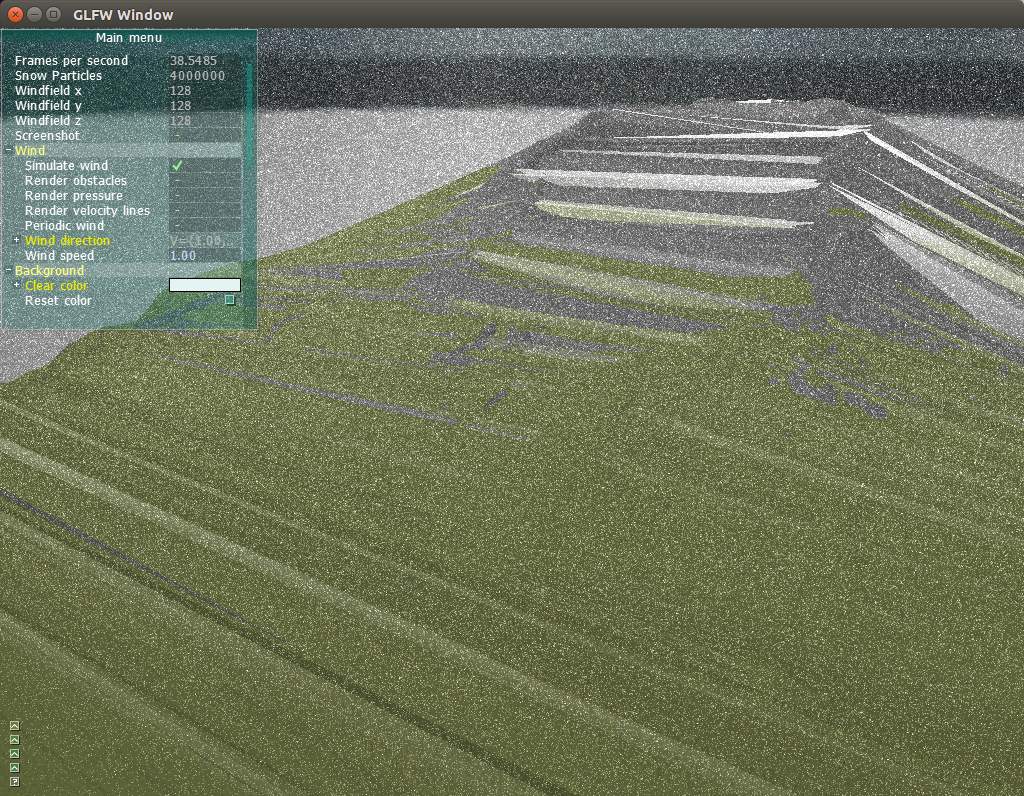
\includegraphics[width=\textwidth]{fig/smoothing}
\caption{Simulator with smoothing function enabled, showing erroneous results.}
\label{fig:smoothing}
\end{figure}

%%=========================================
\subsection{Performance Tests}
Table \ref{table:framerates} contains the frame rates of the CUDA and OpenCL versions for various windfield sizes and particle counts. Profiling data is in the form of a bunch of screen shots, which can be seen in appendix \ref{appendix-b}.

\begin{table}[ht!]
  \begin{center}
    \begin{tabular}{| l | c | c | c |}
    \hline
    \diagbox{Windfield}{Snow particles} & 1 Million & 4 Million & 16 Million \\
    \hline
    32x32x32    & OpenCL: 298 & OpenCL: 113 & OpenCL: 34.0\\
                & CUDA: 336   & CUDA: 126   & CUDA: 45.5 \\
    \hline
    128x128x128 & OpenCL: 99 & OpenCL: 51.1 & OpenCL: 18.1\\
                & CUDA: 93   & CUDA: 52.8   & CUDA: 19.7 \\
    \hline
    256x256x256 & OpenCL: 22 & OpenCL: 17.7 & OpenCL: 10.7\\
                & CUDA: 18   & CUDA: 16.3   & CUDA: 10.4 \\
    \hline

    \end{tabular}
  \end{center}
  \caption{Frame rates for various problem sizes}
  \label{table:framerates}
\end{table}